\subsection{Ricerca area}
Dopo aver cliccato il pulsante \emph{Cerca e visualizza dati} nella schermata Home, verrà visualizzata la schermata di ricerca area:
\begin{figure}[H]
    \centering
    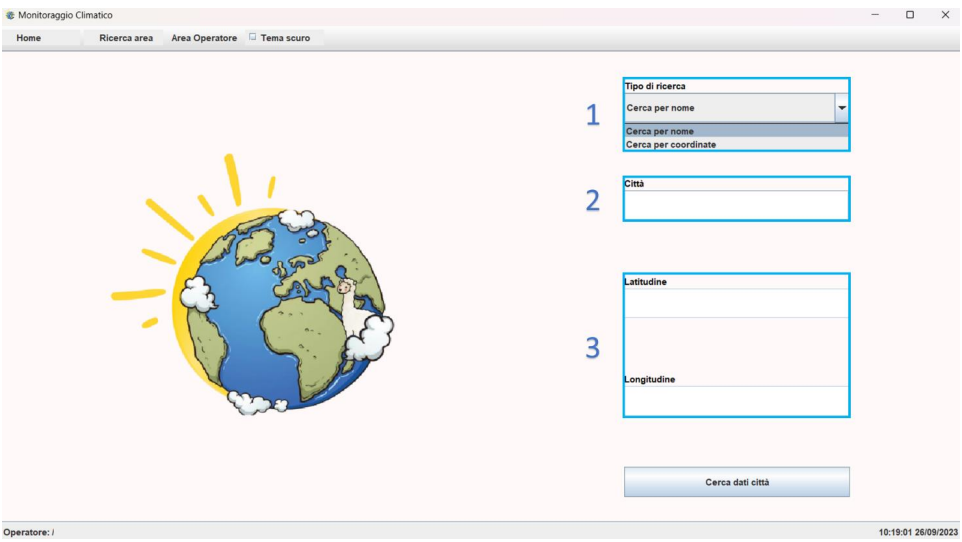
\includegraphics[width=1\textwidth]{../../img/schermata_ricerca_area.png}
    \caption{Schermata Ricerca area}
\end{figure}
Qui è possibile selezionare che tipo di ricerca [1] si vuole effetuare:
\begin{itemize}
    \item \textbf{Ricerca per nome:} permette di cercare un'area speci
    fica inserendo il nome dell'area nell'apposito campo [2].
    \item \textbf{Ricerca per coordinate:} permette di cercare un'area specifica inserendo le coordinate geografiche negli appositi campi [3]
    (Es. 45,123456  9,123456).
\end{itemize}

Quando si clicca il pulsante \emph{Cerca dati città}, se nel sistema sono presenti più città con lo stesso nome o le coordinate insertie fanno riferimento
ad un'area che comprende più città, apparirà un avviso che consente di scegliere la città desiderata: 
\begin{figure}[H]
    \centering
    \includegraphics[width=1\textwidth]{../../img/scelta_città.png}
    \caption{Schermata di scelta della città}
\end{figure} 